\section{Introduction}
\IEEEPARstart{S}{emi-trailer} tank trucks are indispensible for liquid hazardous-chemical logistics, but their  partially filled tanks make rollover a severe safety risk. Accident reports show that tank truck rollovers are often triggered by sharp steering, emergency avoidance, curved-road overspeed, or driver error, and may lead to deadly secondary disasters \cite{chengshuo2023,wangyang2023,wenling_accident2022}. Because safety standards leave practical operation across partial filling rates \cite{biaozhun185642006,biaozhunR00052011}, free-surface sloshing must be considered in autonomous tank truck tracking.

Studies show that with free-surface, driving excitations generate additional sloshing, making medium filling rates yielding stronger dynamic instability than either empty or fully filled cases. And the sloshing in tank has been modeled by quasi-static centroid-shift methods, mechanical equivalent models (MEMs), computational fluid dynamics, and experiments. \cite{maohaijian2021fsi,huangyang2017impact,wanying2020antirolover,wangxiaorun2022lateralacc,chenyibao2016crosssection}. Among the methods, MEMs especially pendulum models are widely used for their ability to balance interpretability and real-time computation, although the dominant sloshing modes still require accurate calibration \cite{jiaxinhong2022review,salem2000rollover,yangxiujian2018multimass,Komasa2023observing}.

For semi-trailer tank trucks, rollover prevention is further complicated by tractor-trailer articulation. High-fidelity models may include lateral, yaw, and roll motion of tractor and trailer,respectively, as well as liquid states \cite{renyuanyuan2020precisemodel,yuzhixin2018mpc,zongchangfu2014identification,niezhigen2015heavyduty}. Such models are useful offline, but online use is limited by trailer replacement, non-unified trailer interfaces, limited trailer-side sensing, and uncertain liquid/suspension parameters. Active suspension, steering, and differential braking have all been studied for rollover prevention \cite{xiao2020rollsuspension,carlson2003rollover,xu2011rollover}; tank truck-specific controllers have used PID, LQR, MPC, model-free adaptive control (MFAC), and other robust control with MEMs \cite{zhaoweiqiang2018equivalent,zhaoweiqiang2019semitrailer,Reviewer2_SunWencai2022,MFAC_LiXiansheng2021,zhao2019hinfty,KomasaQi2025AntiRollover_TITS}.

Most existing controllers still rely on explicit liquid states, roll states, or lateral load transfer ratio (LTR) predictions. This is not always suitable for autonomous semi-trailer tank trucks with limited trailer sensing and embedded computing resources. Model predictive control (MPC) can combine tracking, actuator, acceleration, and safety constraints \cite{gongjianwei2020mpcbook}, but high-dimensional states and dense constraints challenge real-time implementation \cite{shengbo2015fastmpc}. This paper therefore suppresses rollover excitation from the input side: the predicted lateral-acceleration sequence is projected onto vehicle-liquid critical bands, and the resulting energy is penalized and softly constrained. The workflow is shown in Fig.~\ref{fig:intro_architecture}.

\begin{figure*}[!t]
\centering
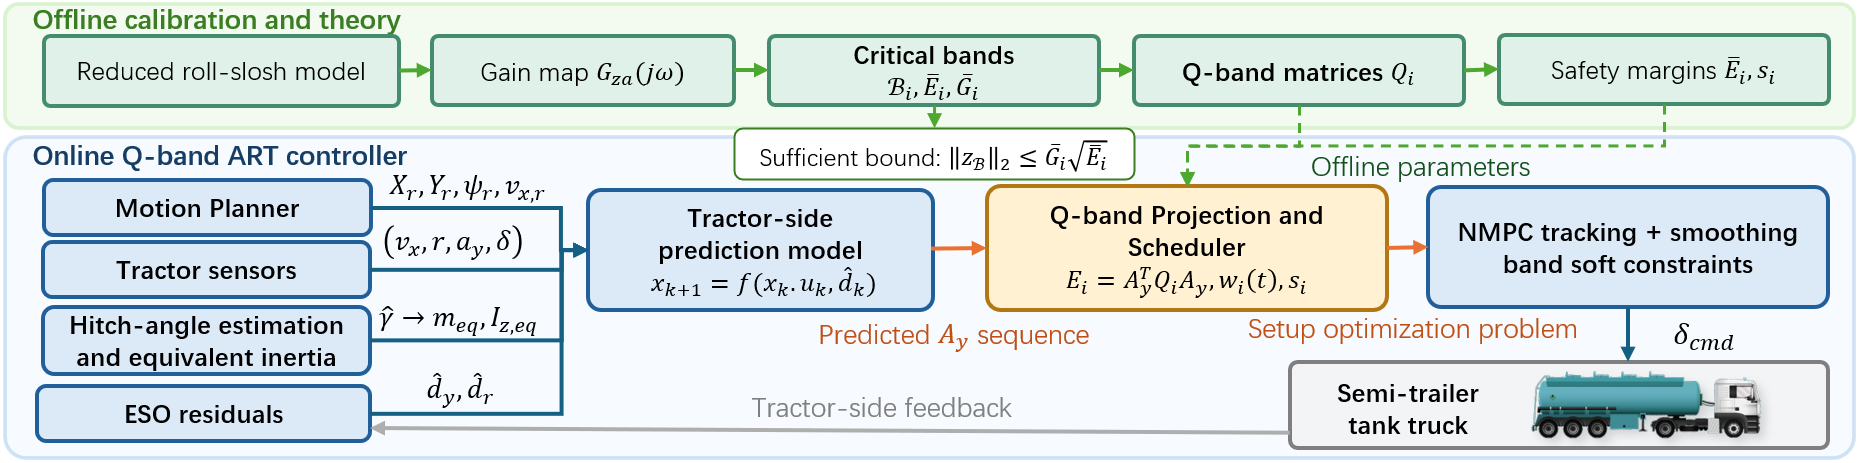
\includegraphics[width=0.98\textwidth]{fig/intro_architecture.png}
\caption{Architecture of Q-band ART. Offline calibration identifies the critical bands, energy thresholds, Q-band matrices, and conservative margins. The online controller then combines tractor-side prediction, ESO residual compensation, hitch-angle-based equivalent-parameter scheduling, Q-band projection, and NMPC to output steering commands using tractor-side sensing and precomputed Q-band parameters.}
\label{fig:intro_architecture}
\end{figure*}


The contributions are threefold. First, a Q-band anti-excitation view is introduced for semi-trailer tank truck tracking, avoiding mandatory online liquid-state modeling and observation. Second, an multi-point NMPC tracking controller with disturbance compensation and trailer-free modeling is designed specifically for semi-trailer. Third, the Q-band term is integrated predictively into the controller for anti-rollover purpose and validated through simulation and 1:14 model-truck experiments. The rest of the paper presents the model, controller, validation, and conclusions. 
